\section{What limits the advantage in practice}
\label{sec:limits}

The diffusion model's advantage at long output is real but thin
($1.4\times$ at $L{=}1024$). The deployment factors that limit it are
severe:

\paragraph{1. Footprint.}

Both models are MoE and have comparable footprints: AR-30B at 60\,GB
vs DG at 52\,GB. Neither can share a GPU with another large model. The
asymmetry that matters is against the quality-similar dense AR-1.5B
(3.0\,GB): 16 copies fit in the space either MoE model occupies.

\paragraph{2. Batching.}

Continuous batching converts arrival concurrency into throughput at
$77\times$ for AR-30B against $\leq 1.7\times$ for DG. Both DG
measurements are engine-bounded (vLLM caps the batch at 8; dInfer
runs cache-less), so the true ceiling is unknown but lies at or above
$1.7\times$. Even so, the gap is more than an order of magnitude
(Appendix~\ref{app:batching}).

\begin{figure}[t]
\centering
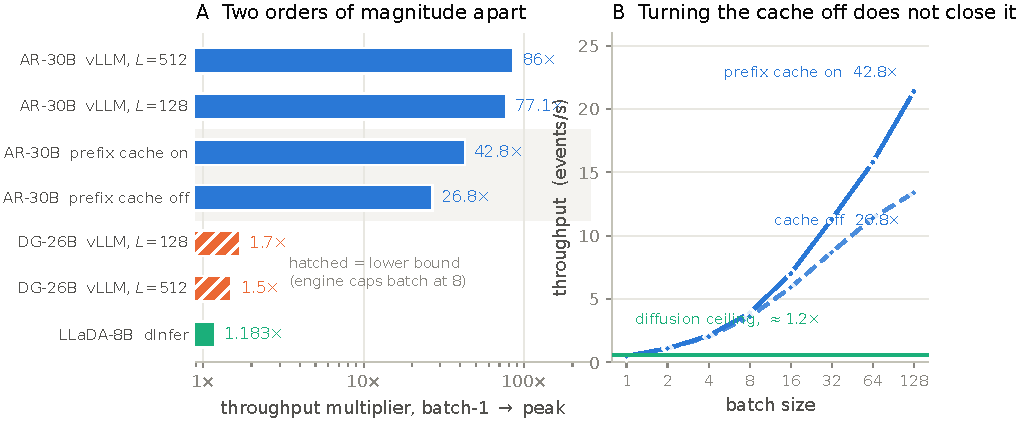
\includegraphics[width=\linewidth]{figures/fig6_batching.pdf}
\caption{Batch-1 to peak throughput multipliers (BGL, $n{=}300$).
AR-30B MoE reaches $77\times$; DG caps at $\leq 1.7\times$.}
\label{fig:batching}
\end{figure}

\paragraph{3. Tail latency.}

The diffusion arm's per-event coefficient of variation is \dgEventCV\%
with a max/median ratio of \dgMaxMed$\times$, against the AR arm's
\arEventCV\% and \arMaxMed$\times$ (Appendix~\ref{app:distributions}).
A $3.21\times$ tail is what breaks a batch-1 SLA --- exactly the
regime where DG's per-event advantage applies.

\paragraph{4. Input length.}

The diffusion prefill slope is \inputSlopeRatio$\times$ steeper than
AR's, because each denoising step re-attends the full prompt. At
longer inputs the base rises and $L^{*}$ moves further upward.

\paragraph{5. Co-residency.}

If batch-1 is imposed by tenant isolation, the relevant alternative is
not the MoE AR-30B but sixteen copies of the quality-similar dense
AR-1.5B (3\,GB each). Per-tenant latency is unchanged; throughput is
$16\times$; isolation is preserved.

\paragraph{Cost per event.}

Table~\ref{tab:cost} prices the comparison at a published on-demand
rate.

\begin{table}[h]
\centering
\caption{Cost per event at three duty cycles. GPU: A100 80GB PCIe at
\$4.62/hr (AWS p4de.24xlarge, August 2026). SXM variants may differ.}
\label{tab:cost}
\begin{tabular}{@{}lrrrr@{}}
\toprule
Arm & Weights & Duty & Events/hr & \$/event \\
\midrule
AR-1.5B (quality-similar) & 3.0\,GB & 100\% & 5{,}408 & \$0.0009 \\
AR-1.5B                   & 3.0\,GB & 25\%  & 1{,}352 & \$0.003 \\
\midrule
DG-26B-A4B                 & 52.0\,GB & 100\% & 9{,}504 & \$0.0005 \\
DG-26B-A4B                 & 52.0\,GB & 25\%  & 2{,}376 & \$0.002 \\
\bottomrule
\end{tabular}
\end{table}

At 100\% duty on a dedicated GPU, the cost ratio is:
\begin{equation}
R_{\mathrm{cost}} = \frac{\$ / \mathrm{event}_{\mathrm{AR}}}
{\$ / \mathrm{event}_{\mathrm{DG}}}
= \frac{0.0009}{0.0005} = 1.8
\end{equation}
where $R_{\mathrm{cost}}$ is the ratio of cost per event between AR
and DG at the same GPU hourly rate. Under co-residency, sixteen
AR-1.5B instances produce $16 \times 5{,}408 = 86{,}528$ events/hr
against DG's 9{,}504. The AR co-resident deployment is $9\times$
cheaper per event while preserving tenant isolation.
